\documentclass[./m2r-pres.tex]{subfile}

\begin{frame}
  \frametitle{RADO'S THEOREM}

  \tikzstyle{box}=[draw, fill=green!20, minimum size=2em]
  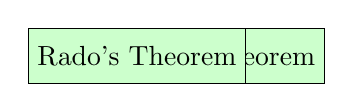
\begin{tikzpicture}
    \node [box] (a) {Rado's Theorem};
    \node [box] (a) [left of=a] {Rado's Theorem};
    
  \end{tikzpicture}

\end{frame}